% !TeX root = ../main.tex
\chapter{架构}\label{ch5}

多年来,深度学习领域已经为每个应用领域开发了多种深度架构,这些架构在多个人们关注的标准方面表现出良好的折中:例如 训练便捷性、预测准确性、内存占用、计算成本、可扩展性等。

\section{多层感知机}\label{sec5.1}

最简单的深度架构是\keyterm{多层感知机}(\keyterm{MLP}),它由一系列\keyterm{全连接层}组成,层与层之间通过\keyterm{激活函数}分隔。请参见图 \ref{fig5.1} 中的示例。由于历史原因,在这样的模型中,\keyterm{隐藏层}的数量指的是线性层的数量,不包括最后一层。

\begin{figure}
    \centering
    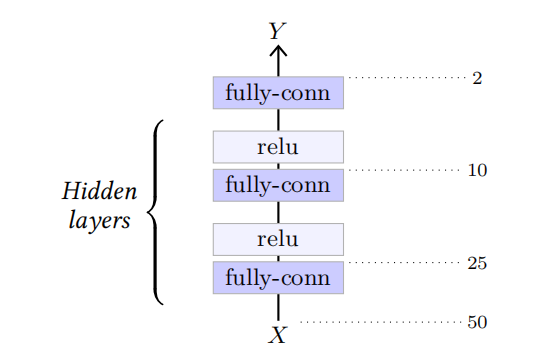
\includegraphics[width=0.9\textwidth]{fig/fig5.1.png}
    \caption[多层感知机]{该多层感知器以大小为 $50$ 的一维张量作为输入,由三个全连接层组成,输出维度分别为 $25$、$10$ 和 $2$,前两个层后面是 ReLU 层。}
    \label{fig5.1}
\end{figure}

一个关键的理论成果是\keyterm{通用逼近定理} \citep{Cybenko1989},该定理指出,如果激活函数 $\sigma$ 是连续的且非多项式的,那么任意连续函数 $f$ 都可以在紧致域上被形式为 $l_2 \circ \sigma \circ l_1$ 的模型任意精确地一致逼近,其中紧致域是有界的并包含其边界,$l_1$ 和 $l_2$ 是仿射的。这样的模型是一个只有单个隐藏层的多层感知机(\keyterm{MLP}),这个结果意味着它可以近似任何具有实用价值的东西。然而,这种逼近成立的条件是第一个线性层的输出维度可以任意大。

尽管 MLP 很简单,但当要处理的信号维度不太大时,它仍然是一个重要的工具。

\section{卷积网络}\label{sec5.2}

\section{注意力模型}\label{sec5.3}